\chapter{传输层}

\noindent\textbf{本章要解决的问题。} 网络层把IP数据报送到目标主机；传输层还要把收到的数据交给主机中的正确应用进程，并按应用需要提供服务。本章按课件顺序学习：进程之间的逻辑通信、端口与套接字、UDP、可靠数据传输、TCP连接与字节流，以及TCP的流量控制和拥塞控制。

\section{传输层服务}
\textbf{进程}是正在运行的程序及其状态。网页浏览器、邮件程序和视频应用可以同时运行在同一台主机上。网络层主要识别\textbf{主机}，传输层再依据端口等信息把数据交给主机中的\textbf{进程}。因此，传输层提供的是端系统之间进程到进程的逻辑通信。

发送端的封装顺序是：应用数据加上传输层首部，形成TCP报文段或UDP数据报；再装入IP数据报，最后封装成链路层帧。接收端按相反方向逐层去掉首部并交付。传输层首部中的端口帮助分用；IP首部中的协议号帮助网络层区分TCP、UDP等上层协议。

传输控制协议TCP（Transmission Control Protocol）和用户数据报协议UDP（User Datagram Protocol）提供不同服务。TCP面向连接，提供可靠、按序的字节流，并带有接收端流量控制与网络拥塞控制；UDP无连接、首部短，不保证交付、按序或不重复。应用可以根据需要在UDP之上自己实现确认和重传。传输层协议运行在端系统上，路由器通常只处理IP层及以下的转发。

\annotationarea[4]
\small 来源：课件 \texttt{Chapter5-传输层.pdf}，PDF阅读器第3--8页；PDF第3页显示页为3，PDF第4--8页无独立显示页码。参考书PDF第235--236页（印刷第224--225页）。\normalsize

\section{多路复用与分用}
\textbf{多路复用}发生在发送端：多个应用进程把数据交给传输层，传输层分别加上端口等首部，再把报文交给网络层。\textbf{分用}发生在接收端：传输层检查收到报文段的首部，并将数据交给相应套接字。

\textbf{端口号}是传输层用于识别通信端点的16位数字。\textbf{套接字}是应用进程与传输层交互的端点；它会和本地地址、端口及协议等信息关联。端口数值在TCP与UDP中可以分别使用。

\begin{itemize}[nosep]
\item \textbf{UDP分用：}课件模型以目的IP地址和目的端口找到接收套接字；同一个UDP服务器端口可以接收来自多个客户端的数据报。应用仍能从每个数据报中读到源IP与源端口，以便回复。
\item \textbf{TCP分用：}已建立的连接通常由源IP、源端口、目的IP、目的端口四元组区分。多个客户端可以同时连接同一服务器IP和服务端口，因为每个连接的客户端端点不同。监听套接字负责接收新连接，建立后的连接由各自的连接套接字处理。
\end{itemize}

\begin{center}\begin{tabular}{lll}\toprule 传输协议 & 课件中的主要分用信息 & 同一服务端口能否接收多客户端\\\midrule
UDP & 目的IP地址、目的端口 & 可以，同一UDP套接字可收到多个源的数据报\\
TCP & 源/目的IP地址、源/目的端口四元组 & 可以，每条连接有独立四元组\\\bottomrule\end{tabular}\end{center}
\annotationarea[4]
\small 来源：课件PDF阅读器第9--17页；PDF第9、15、17页分别显示页9、15、17，PDF第10--12页无独立显示页码。参考书PDF第236--238页（印刷第225--227页）。\normalsize

\section{UDP用户数据报协议}
\subsection{UDP提供什么服务}
UDP（用户数据报协议）无须在发送数据前建立连接。发送方每次独立发送一个数据报，接收方可能收不到、收到乱序数据，或收到重复数据；UDP本身不自动重传，也不保证数据交付给应用。DNS查询、SNMP和部分实时音视频会使用UDP。应用如果需要可靠性，可在应用层增加确认、重传或特定错误恢复。

UDP首部固定8字节，由源端口、目的端口、长度、校验和四个各2字节的字段组成。长度以字节计，包含UDP首部与数据，不含IP首部。例如应用数据100字节，则UDP长度字段为108字节。

\subsection{UDP校验和的计算}
校验和用于发现传输中可能发生的位错误，不负责修复错误。IPv4的计算范围包含伪首部、UDP首部和应用数据。\textbf{伪首部}临时取自IP层的源/目的地址、协议号17和UDP长度，参与计算但不作为独立字段发送。若数据字节数为奇数，只在计算时末尾补一个0字节。

计算步骤：把校验和字段先置0；将待检内容按16位分组；用反码加法相加，把最高位的进位回卷到最低位；将最终和逐位取反，作为校验和。接收方按相同方式把校验和也纳入求和，结果全1表示未检测到错误，不代表绝对没有错误。

\textbf{课件手算例（PDF第23页）。} 课件给出两个16位字：
\[
1110011001100110\quad(\texttt{0xE666}),\qquad
1101010101010101\quad(\texttt{0xD555}).
\]
分步计算：
\[
\begin{aligned}
\texttt{0xE666}+\texttt{0xD555}&=\texttt{0x1BBBB},\\
\text{回卷最高位进位：}\quad\texttt{0xBBBB}+1&=\texttt{0xBBBC},\\
\text{逐位取反：}\quad\texttt{0xBBBC}&\longrightarrow\texttt{0x4443}
 = \texttt{0100010001000011}.
\end{aligned}
\]
因此校验和值为$\texttt{0x4443}$。若数据字更多，就继续逐个相加并回卷每次产生的进位。\annotationarea[4]
\small 来源：课件PDF阅读器第18--23页；PDF第19页显示页3，PDF第20--23页显示页与PDF页相同。参考书PDF第240--242、245页（印刷第229--231、234页）。\normalsize

\section{可靠数据传输}
\subsection{可靠交付需要哪些机制}
可靠交付的目标是：数据不错、不丢、不乱、不多。底层信道可能损坏、丢失或延迟分组，协议因此需要校验和、确认、序号、重传和定时器。课件用有限状态机描述发送方、接收方在不同事件后的动作；状态表示当前协议进展，事件可能是收到分组、收到确认、校验失败或定时器超时。

\begin{itemize}[nosep]
\item \textbf{rdt 1.0：}假设底层信道完全可靠，发送方发出、接收方交付即可。
\item \textbf{rdt 2.0：}考虑分组位错误；用校验和检错，接收方以ACK（acknowledgment，确认）确认正确分组，以NAK（negative acknowledgment，否定确认）报告损坏，发送方收到NAK后重传。基于确认和重传的机制称自动重传请求（ARQ，Automatic Repeat reQuest）。
\item \textbf{rdt 2.1：}ACK或NAK也可能损坏。发送方给数据分组加0/1序号；接收方根据期望序号识别重复分组，避免把重传数据重复交给应用。
\item \textbf{rdt 2.2：}不单独发NAK；接收方重复确认最近正确收到的分组。发送方收到不匹配的重复ACK时重传当前分组。
\item \textbf{rdt 3.0：}数据分组或确认都可能丢失或延迟；发送方启动定时器，若超时仍没有有效确认就重传。序号让接收方识别延迟到达的旧分组。
\end{itemize}

\textbf{事件例：ACK丢失。} 发送方发送序号0并启动计时器；接收方校验正确后向应用交付一次，并返回ACK0；ACK0在途中丢失。发送方超时重发序号0，接收方发现自己当前期待序号1，于是丢弃重复数据、再次回ACK0；发送方收到确认后再发送序号1。若没有序号，接收方无法分辨重传分组和新的相同数据。

\textbf{事件例：分组丢失。} 发送方发序号1后启动定时器；分组未到达，接收方没有可确认的数据；定时器到期，发送方重新发送序号1；接收方收到并交付一次，再回ACK1。

\textbf{事件例：定时器过早触发。} 发送方发出分组1，分组已经到达接收方并被交付，但ACK1返回较慢。发送方在ACK回来前超时并重发1；接收方按序号认出这是重复分组，不再次交付，只重发ACK1。发送方收到一个有效ACK后继续发下一个新分组。过早超时会产生多余重传，但序号避免了重复交付。

\annotationarea[4]
\small 来源：课件PDF阅读器第24--44页（该组课件页脚编号通常与PDF页相同）；参考书PDF第72--78页（印刷第61--67页）。\normalsize

\subsection{停等协议与流水线}
\textbf{停等}表示每发送一个分组，发送方都要等确认回来，之后才能发下一个。设分组长度为 $L$ bit，链路速率为 $R$ bit/s，则发送一个分组的时间为 $t_{\rm seg}=L/R$。RTT（Round-Trip Time，往返时间）在此按数据最后一位发出到ACK第一位回来计；ACK发送时长为 $t_{\rm ACK}$。忽略处理、排队和错误，则信道利用率为
\[
U_{\rm stop}=\frac{t_{\rm seg}}{t_{\rm seg}+\mathrm{RTT}+t_{\rm ACK}}.
\]

\textbf{课件例（PDF第45--47页）：}链路速率1 Gb/s、单程传播时延15 ms、数据分组1 KB，忽略ACK发送时长。若1 KB按1000 B计，分组发送时间为 $8000/10^9=8\,\mu s$；往返传播时间约30 ms。因此
\[
U\approx\frac{8\,\mu s}{30\,ms+8\,\mu s}\approx0.0267\%.
\]
发送方约每30 ms才能发出一个1 KB分组，所以平均数据速率约为$8{,}000\text{ bit}/0.030\text{ s}=267\text{ kb/s}$，即约33 KB/s，远低于链路容量。限制在于协议等待时间，而非物理链路速率。

\textbf{流水线}允许发送方在收到确认之前连续发多个分组。发送窗口大小 $W_s$ 表示最多可有多少个分组处于未确认状态。在理想无损、等长分组、ACK可忽略且接收端能够持续接收时，近似利用率为
\[
U\approx\min\left(1,\frac{W_s t_{\rm seg}}{t_{\rm seg}+\mathrm{RTT}+t_{\rm ACK}}\right).
\]
窗口增大可提升利用率，但也需要更大的序号空间与缓存，并受到流量控制和拥塞控制限制。

\annotationarea[4]

\subsection{GBN：累积确认，超时后退回重传}
\textbf{后退N帧（GBN）}发送方最多有 $N$ 个未确认分组在途。ACK(n)表示截至序号$n$（包含$n$）的分组都已正确收到，这是\textbf{累积确认}。接收方只接收当前期待的序号；若收到乱序分组，丢弃它并重复确认最近连续收到的序号。发送方通常为最早未确认分组维护一个定时器；超时后重发该分组及其后所有尚未确认的分组。

\textbf{课件例（PDF第59页）：}发送方已发序号0到7，收到ACK0、ACK2、ACK3。由于ACK3累计确认0到3，当前最早未确认分组是4。若此时定时器超时，重发4、5、6、7，共4帧。注意GBN的ACK(n)含义是“到n为止都收到”，TCP中的ACK号含义不同，见后文。

若序号字段为$k$位，序号空间大小是$2^k$；GBN的接收窗口为1，发送窗口最大为$2^k-1$，留出一个序号以避免新旧分组混淆。

\annotationarea[4]

\subsection{SR：逐个确认，重传缺失分组}
\textbf{选择重传（SR）}接收方分别确认每个分组，可缓存窗口内的乱序分组；发送方为未确认分组分别设定时器，超时只重发对应分组。接收方仍按序向上交付：当缺失的分组到达后，它可以把该分组及缓存中紧跟其后的连续分组依次交付。

\textbf{课件事件例（PDF第64页）：}发送窗口大小4，先发送0、1、2、3，其中2丢失。接收方交付0和1，分别回ACK0、ACK1；收到3时先缓存并回ACK3。发送方收到ACK0后发4，收到ACK1后发5；4和5到达后，接收方继续缓存并分别回ACK4、ACK5。随后2的计时器超时，发送方只重发2；接收方收到2后按序交付2、3、4、5，并滑动接收窗口。这个例子显示SR避免像GBN那样重复发送已经到达的3、4、5。

\begin{figure}[H]\centering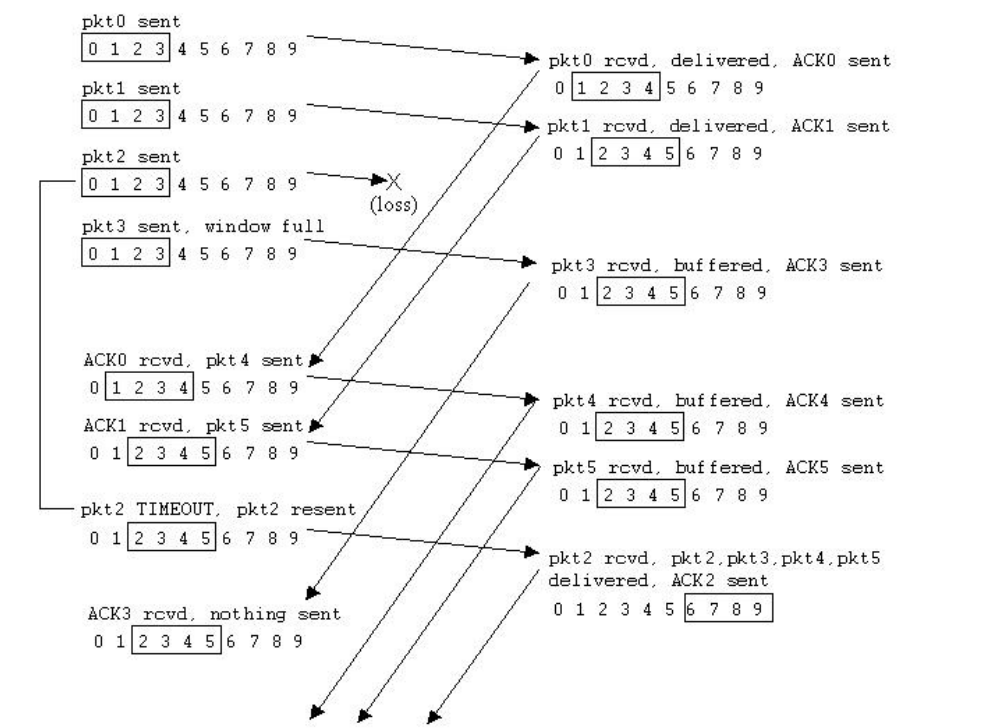
\includegraphics[width=.94\textwidth]{ch05-sr-example.png}\caption{选择重传的事件序列：2号分组丢失，接收方缓存3、4、5，发送方超时后只重传2。来源：Chapter5-传输层.pdf，PDF第64页（显示页64），局部截取。}\end{figure}

\textbf{序号空间限制。} 如果序号空间有$M=2^k$个值，发送窗口为$W_s$、接收窗口为$W_r$，为避免窗口回绕后把旧分组认成新分组，常见条件是$W_s+W_r\le M$。典型等大小SR窗口满足$W_s=W_r=W$，因此$W\le M/2=2^{k-1}$；停等的窗口均为1，至少需要1位序号。

\textbf{课件困境例（PDF第65--66页）：}序号为0、1、2、3，窗口大小3。发送端发送旧的序号0后，若它延迟很久；接收端先收到1、2并滑动窗口，再进入下一轮窗口0、1、2。此时旧序号0和新一轮序号0对接收端看起来相同，接收端可能把旧数据误当新数据交付。窗口3超过序号空间一半（2），无法仅凭序号消歧，因此SR窗口需满足上面的限制。

\annotationarea[4]
\small 来源：课件PDF阅读器第49--67页；参考书PDF第72--78页（印刷第61--67页）。\normalsize

\section{TCP：连接、字节流与首部}
\subsection{TCP提供面向连接的字节流}
TCP在两端建立连接状态后传送数据，提供全双工通信：两个方向可同时传数据，每个方向有各自的序号。\textbf{字节流}表示TCP把应用写入的数据看成连续字节，不保留每次写入的消息边界。一次写入100 B，对端可能分几次读取，也可能与后续写入一起读；应用若需要消息边界，必须自行定义长度或分隔符。

发送和接收两端都使用缓存。发送缓存保存尚未确认的数据以便重传；接收缓存暂存按序数据并等待应用读取。TCP的可靠性意味着协议会检测丢失、损坏和重复并尝试恢复；若连接长期不能恢复，应用仍可能收到错误。

\subsection{TCP首部和字节序号}
TCP首部固定部分为20 B；选项和填充可使首部最长达到60 B。数据偏移字段以4 B为单位表示首部长度，例如值5表示20 B。\textbf{MSS}是一个TCP段可携带的最大数据字节数，不包括TCP/IP首部。

\begin{figure}[H]\centering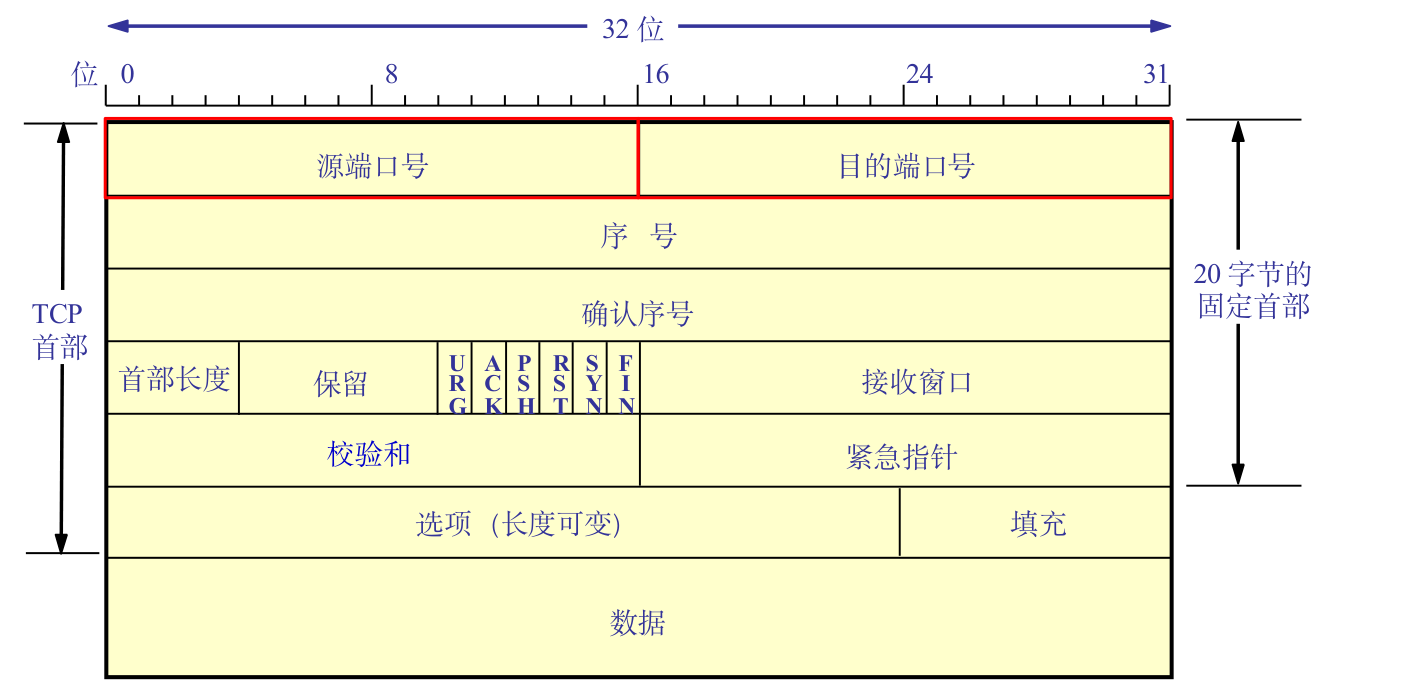
\includegraphics[width=.88\textwidth]{ch05-tcp-header.png}\caption{TCP基本首部字段布局，每行32 bit。来源：\texttt{Chapter5-传输层.pdf}，PDF第70页（显示页70），局部截取。}\end{figure}

\begin{center}\small\setlength{\tabcolsep}{4pt}
\begin{tabularx}{\textwidth}{>{\raggedright\arraybackslash}p{2.8cm}>{\centering\arraybackslash}p{1.2cm}>{\raggedright\arraybackslash}X}
\toprule 字段 & 位数 & 作用\\\midrule
源端口、目的端口 & 各16 & 标明两端应用进程的传输层端点\\
序号、确认号 & 各32 & 标明本段首字节编号，以及下一步期待收到的字节编号\\
数据偏移、保留、控制位 & 4、6、6 & 表示首部长度；保留位供协议扩展；经典控制位含URG、ACK、PSH、RST、SYN、FIN\\
接收窗口 & 16 & 通告接收方当前可接收的字节范围\\
校验和、紧急指针 & 各16 & 检错；URG有效时紧急指针标记紧急数据末端\\
选项与填充 & 可变 & 可携带MSS、时间戳、SACK等；填充使首部长度对齐到4 B\\\bottomrule
\end{tabularx}\end{center}

源端口和目的端口各16位；序号seq标明本段第一个数据字节的编号；确认号ack在ACK标志置位时有效，表示接收方\textbf{下一步期待的字节编号}。若接收方已连续收到截至400的字节，ack为401。接收窗口rwnd以字节通告接收端当前可用空间。校验和保护伪首部、TCP首部和数据；SYN用于同步连接两端的序号，FIN表示本方向发送结束，RST复位连接。PSH、URG及选项等字段按具体需要使用。TCP序号按$2^{32}$模回绕；SYN和FIN各占一个序号，纯ACK不消耗数据序号。

\textbf{课件序号例：}A发送seq=301、载荷100 B，则字节301--400被发送。若此前字节均连续收到，B回复ack=401。若A发送seq=401--500的数据段丢失，而后面的501--600到达，B仍回复ack=401，因为它期待的下一个连续字节仍是401。收到缺口后面的数据不等于确认了缺失字节。

课件PDF第80页另用单字节演示双向编号：A发seq=42的1 B，B确认ack=43；B用自己的序号空间发seq=79的1 B，A确认ack=80。两端各自维护发送序号，因此A的seq与B的seq不要求相等。

\textbf{GBN与TCP确认号的区别：}GBN的ACK(n)确认序号为$n$的分组以及此前分组；TCP的ack=$n$表示$n$之前的连续字节已收到、下一步期待字节$n$。两者都具有累计确认效果，但编号单位和字段含义不同。

\annotationarea[4]
\small 来源：课件PDF阅读器第68--80页；参考书PDF第247--249页（印刷第236--238页）。\normalsize

\section{TCP可靠传输与流量控制}
\subsection{确认、超时与快速重传}
TCP发送端缓存已发但尚未确认的数据，按累计确认推进最早未确认字节；接收端通常对连续收到的字节回复累计ACK。若ACK迟迟未到，发送端超时后重传最早未确认数据。

\textbf{快速重传}利用重复ACK及早发现缺口。例：接收方已收到字节0--999，下一段1000--1099丢失；之后三个更高序号的数据段到达，接收方仍发ack=1000。发送方收到三个重复ack=1000后，可立即重传从1000开始的数据段，不必等超时。重复ACK是丢失的线索，但也可能由乱序触发。

\textbf{RTT测量与重传超时。} SampleRTT是某数据段发出至其确认返回的测量值。段发生重传后，确认可能对应原发送或重传，来源不确定，通常不把这种样本用于估计。课件用指数加权平均计算：
\[
EstimatedRTT\leftarrow(1-\alpha)EstimatedRTT+\alpha SampleRTT,
\]
\[
DevRTT\leftarrow(1-\beta)DevRTT+\beta|SampleRTT-EstimatedRTT|,
\]
\[
TimeoutInterval=EstimatedRTT+4DevRTT.
\]
课件典型参数为$\alpha=0.125$、$\beta=0.25$。估计偏差越大，超时等待留出的余量越大。实际TCP还会使用计时器粒度、上下限和超时退避等细节。

\annotationarea[4]

\subsection{接收窗口与流量控制}
\textbf{流量控制}防止发送方把接收缓存填满，使接收应用有时间读取数据。接收方在TCP首部中通告rwnd；发送方在途未确认数据和新数据合计不能超过接收方允许的窗口。简化描述中，若接收缓存容量为$B$字节，缓存中尚未被应用读取的数据为$Q$字节，则$rwnd=B-Q$。

\textbf{例：}接收缓存容量4000 B，其中1000 B尚未被应用读取，则当前通告空间为3000 B。若发送窗口中已有1500 B未确认，接收端新空间为3000 B，则最多再发送1500 B，避免累计占用超过3000 B。若发送窗口为0，发送端暂停普通新数据；窗口更新可能丢失，TCP可用持续计时器和零窗口探测确认窗口是否重新开放。

\textbf{流量控制与拥塞控制的区别：}rwnd反映接收主机的可用缓存；cwnd反映发送端对网络可承受数据量的估计。简化模型允许未确认数据量不超过$\min(rwnd,cwnd)$；还需扣除已经在途的未确认数据，才得到当前可新发送的字节数。

\annotationarea[4]
\small 来源：课件PDF阅读器第81--92页；参考书PDF第252--254页（印刷第241--243页）。\normalsize

\section{TCP连接建立与释放}
\subsection{三次握手}
建立连接前，双方需要交换各自的初始序号并建立连接状态。设客户端初始序号为$x$、服务器为$y$：
\begin{enumerate}[nosep]
\item 客户端发SYN，seq=$x$。SYN占用一个序号，客户端进入SYN\_SENT。
\item 服务器回SYN+ACK，seq=$y$、ack=$x+1$，进入SYN\_RCVD。
\item 客户端回ACK，seq=$x+1$、ack=$y+1$。服务器收到后双方连接建立；第三段也可携带数据。
\end{enumerate}

\begin{figure}[H]\centering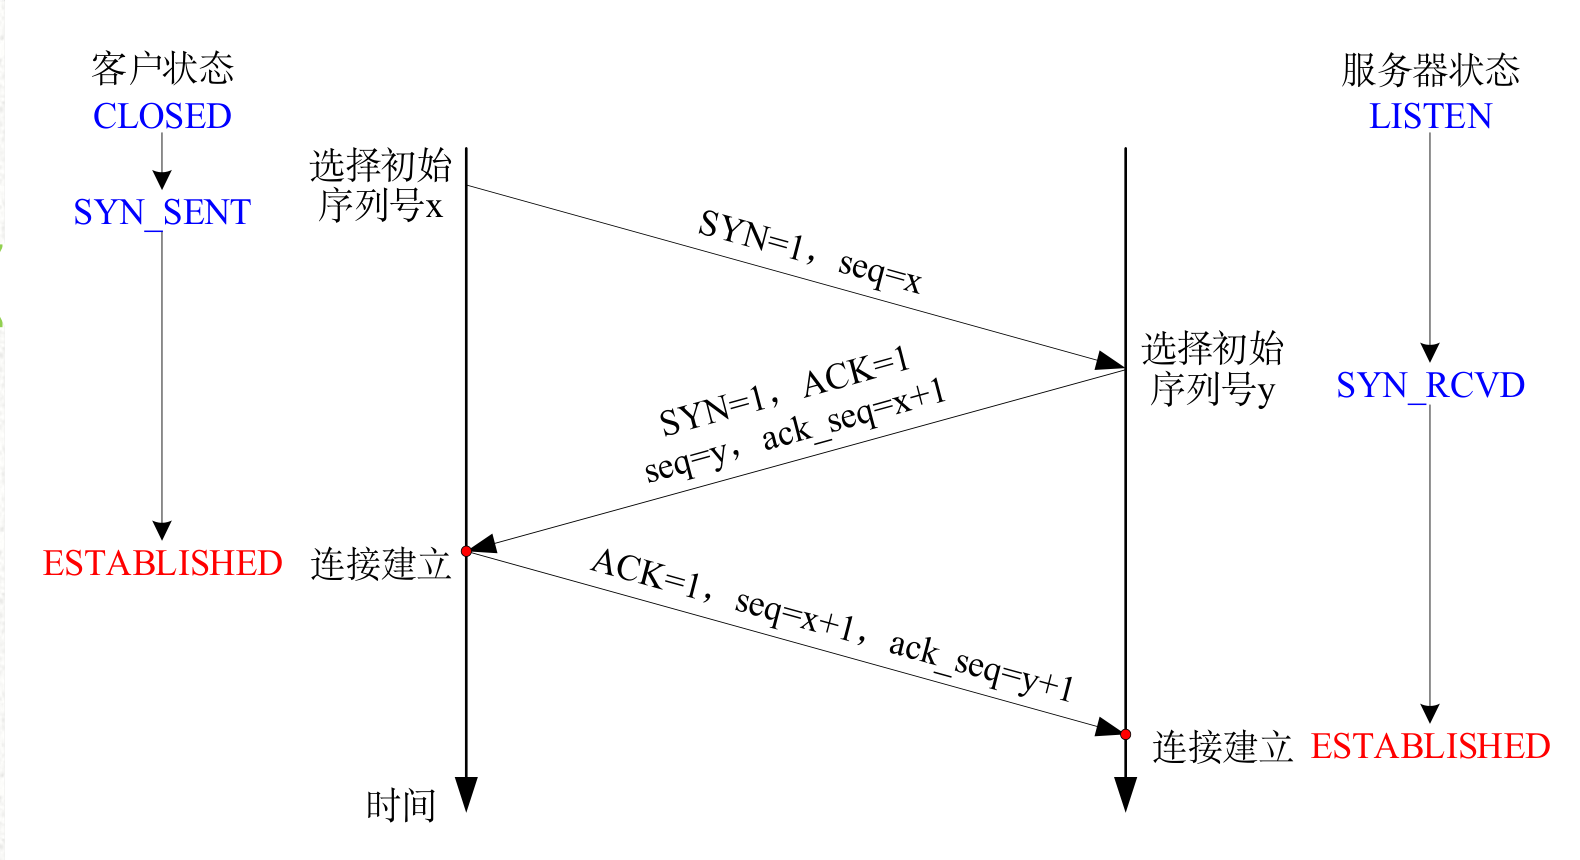
\includegraphics[width=.86\textwidth]{ch05-handshake.png}\caption{三次握手的报文顺序、序号确认和连接状态。来源：\texttt{Chapter5-传输层.pdf}，PDF第94页（显示页94），局部截取。}\end{figure}

图中两条竖线分别代表客户端和服务器，时间自上向下，斜箭头表示报文方向。第三次握手使服务器知道客户端收到了自己的初始序号，并帮助区分迟到的旧SYN和新连接。最终ACK到达之前服务器可能保留半连接状态，因此握手不能避免所有资源消耗。

\subsection{关闭连接与半关闭}
TCP是全双工的。一方发FIN只表示自己不再发送新数据，另一方向仍可能继续传数据，所以关闭常见为四个控制报文：
\begin{enumerate}[nosep]
\item 主动关闭方发FIN，进入FIN\_WAIT\_1；FIN占一个序号。
\item 被动方回ACK，进入CLOSE\_WAIT；主动方收到后进入FIN\_WAIT\_2。此时主动方还能接收对方数据，这种状态称半关闭。
\item 被动方完成发送后发FIN，进入LAST\_ACK。
\item 主动方回ACK并进入TIME\_WAIT；被动方收到后关闭。主动方等待$2MSL$后关闭，MSL表示报文段最大生存时间。
\end{enumerate}

\begin{figure}[H]\centering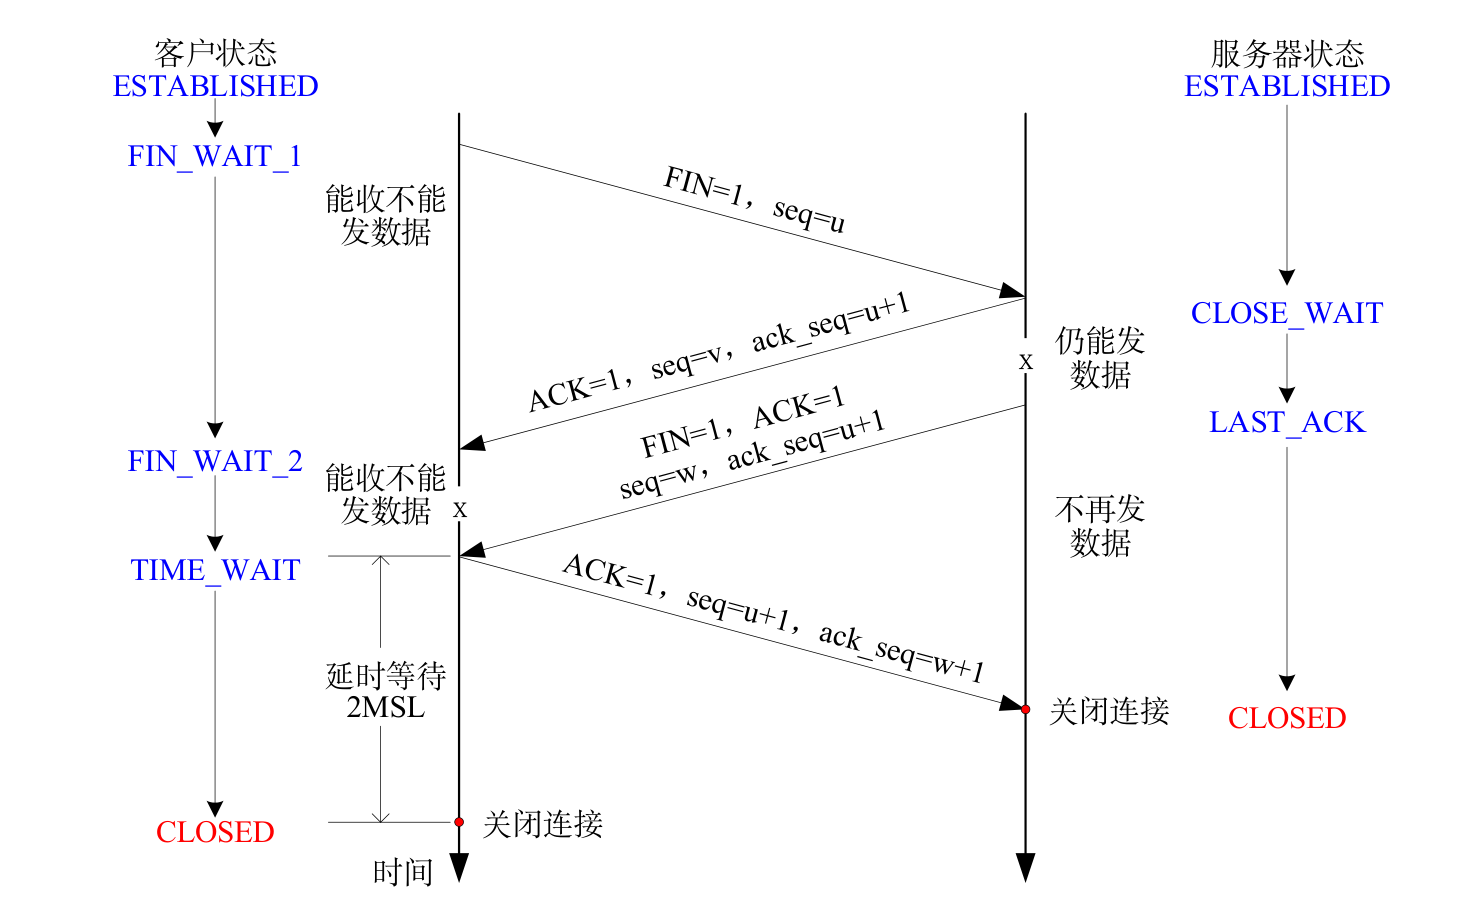
\includegraphics[width=.84\textwidth]{ch05-close.png}\caption{主动方与被动方关闭连接的报文及状态变化。来源：\texttt{Chapter5-传输层.pdf}，PDF第96页（显示页96），局部截取。}\end{figure}

ACK可与对方FIN合并，因此实际报文数并非必定正好四个。TIME\_WAIT等待可在最后ACK丢失时重新确认对方重传的FIN，并让旧报文从网络中消失。

\annotationarea[4]
\small 来源：课件PDF阅读器第93--97页；参考书PDF第249--251页（印刷第238--240页）。\normalsize

\section{TCP拥塞控制与性能}
\subsection{cwnd、慢启动与拥塞避免}
拥塞指网络中注入的流量超过某些链路或路由器的处理能力，排队时延会增长，缓存满时会丢包。TCP发送端看不到所有路由器内部状态，因此用丢包、超时、重复ACK或显式拥塞通知等信号调整发送速率。

\textbf{拥塞窗口cwnd}限制已发出但尚未确认的数据量，用来控制进入网络的流量。若发送方始终有数据、接收窗口足够且无其他瓶颈，粗略发送速率约为$cwnd/RTT$字节/秒。MSS是每段最大数据量，ssthresh是慢启动门限。

\begin{itemize}[nosep]
\item \textbf{慢启动：}课件教学模型初始cwnd为1 MSS；每收到一个新确认的满尺寸段，cwnd约增加1 MSS。因此在一个RTT内收到多个ACK时，cwnd约翻倍：1、2、4、8 MSS。课件例以MSS=500 B、RTT=200 ms起步，初始速率为$500\times8/0.2=20{,}000$ bit/s，即20 kb/s。慢启动的初始窗口小，但增长是指数式的。
\item \textbf{拥塞避免：}达到门限后，约每RTT增加1 MSS，即线性增长。课件用逐个ACK的小幅调整实现这一增长。
\item \textbf{丢包后的窗口调整：}三个重复ACK表示仍有数据在网络中传输，课件模型把ssthresh设为丢失时cwnd的一半，再执行快速重传并进入拥塞避免；超时被视为更严重拥塞，ssthresh设为原cwnd的一半、cwnd降至1 MSS，再进入慢启动。算法版本和教学模型的细节可能不同，做题时应按题目给定规则。
\end{itemize}

\begin{figure}[H]\centering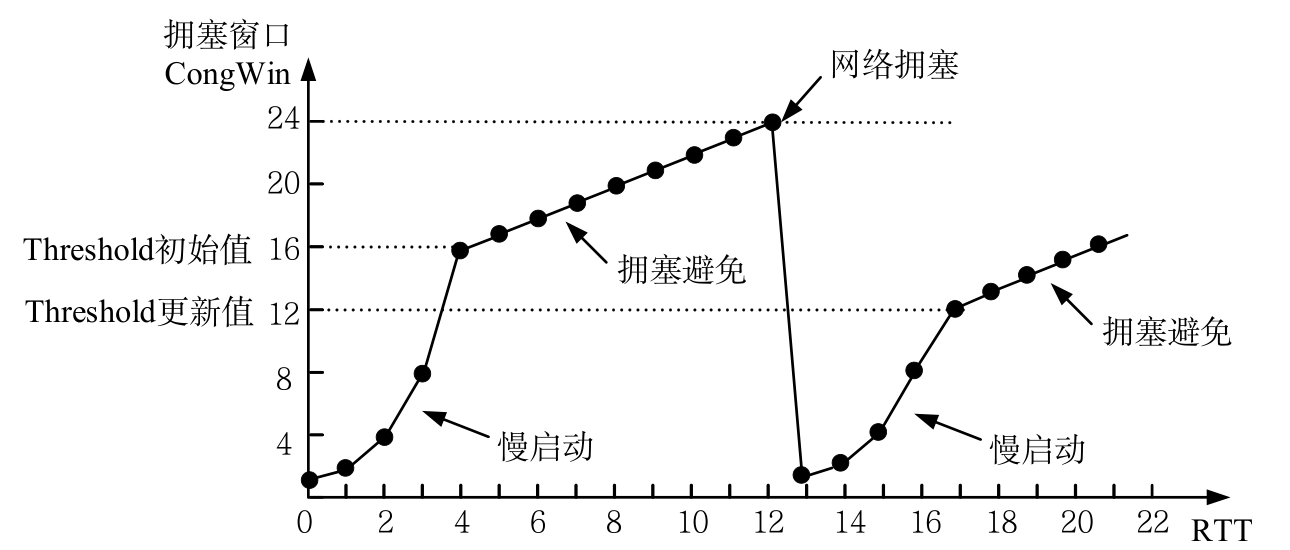
\includegraphics[width=.82\textwidth]{ch05-congestion.png}\caption{慢启动、拥塞避免及丢包后的窗口变化示意。来源：\texttt{Chapter5-传输层.pdf}，PDF第103页（显示页103），局部截取。}\end{figure}

\textbf{课件例题（PDF第108页）：}MSS=1 KB，cwnd=16 KB时发生超时。新门限为$16/2=8$ KB，cwnd回到1 KB。若之后各段都成功确认，慢启动每RTT约翻倍：第1个RTT后2 KB，第2个后4 KB，第3个后8 KB；达到门限后转为拥塞避免，第4个RTT结束时增加约1 KB至9 KB。

\subsection{快速恢复及其他拥塞信号}
TCP Reno教学模型收到三个重复ACK后，把门限设为原窗口的一半，并令cwnd暂时膨胀为$ssthresh+3MSS$；每多收到一个重复ACK，可再临时增加约1 MSS；收到确认新数据的ACK后，cwnd回到ssthresh并进入拥塞避免。窗口临时膨胀是因为重复ACK意味着有数据仍离开网络。发生超时则按更严重拥塞处理：cwnd回到1 MSS，重新慢启动。

课件还介绍：
\begin{itemize}[nosep]
\item \textbf{TCP CUBIC：}以曾发生丢包时的窗口$W_{max}$为参考，丢包后较快增长，接近$W_{max}$时放慢探测；窗口增长与距目标时刻$K$的时间差的立方相关。
\item \textbf{基于时延的拥塞控制：}以RTT增长作为队列可能变长的信号，目标是让瓶颈链路保持繁忙，同时避免缓存排队过多。最低观测RTT记为$RTT_{min}$，用$cwnd/RTT_{min}$估计无拥塞时的吞吐率，再与实测吞吐率比较，判断是否继续增加窗口。
\item \textbf{ECN显式拥塞通知：}支持ECN的路由器可在IP首部的ECN位标记拥塞；接收端在TCP确认中设置ECE等标志通知发送方，发送方据此降低发送速率。该机制需要网络和端系统共同支持。
\end{itemize}

\subsection{吞吐率、丢包率与公平性}
固定拥塞窗口为$W$个MSS、RTT稳定且发送方总有数据时，吞吐率近似为
\[
Throughput\approx\frac{W\times MSS\times8}{RTT}\quad\text{bit/s}.
\]
\textbf{课件例（PDF第110页）：}MSS=1500 B、RTT=100 ms，希望达到10 Gb/s，则
\[
W=\frac{10^{10}\times0.1}{1500\times8}\approx83{,}333\text{ 段}.
\]
该窗口代表需要同时在途的大量数据，尚未计入协议首部等开销。

课件PDF第109页给出的锯齿窗口近似为平均吞吐率$0.75W/RTT$：假设窗口在$W/2$与$W$之间线性增长，均值为$3W/4$，再除以RTT。课件该页把减半与“超时”相连，但第104--106页明确说超时将cwnd降至1 MSS；因此$0.75W/RTT$应理解为忽略慢启动、按稳定的加性增大/乘性减小锯齿周期得到的近似，不能把它当成每次超时之后的精确吞吐率。

\textbf{课件丢包率例（PDF第111页）：}窗口由$W/2$逐步增加至$W$时发送的段数近似为
\[
W/2+(W/2+1)+\cdots+W\approx3W^2/8+3W/4.
\]
当$W$较大时主项为$3W^2/8$，若该周期发生一个丢包，则丢包率近似$L\approx8/(3W^2)$。这是忽略低阶项的近似关系。

在理想公平模型中，$K$条特征相似、共享容量为$R$的TCP连接各自平均获得约$R/K$。实际结果受RTT、算法、路径和发送需求影响。课件例中已有9条连接：新应用只开1条TCP连接，约分得$R/10$；若开11条并行连接，课件近似写作$R/2$。按每条连接均分的简化假设，11条连接合计为$11R/20\approx0.55R$，与课件的$R/2$近似接近。这说明按连接公平不一定等于按应用公平。实际结果也会受实现和网络影响。若应用不做拥塞控制而用UDP持续高速发送，也可能挤占TCP流量。

\annotationarea[4]
\small 来源：课件PDF阅读器第98--123页；参考书PDF第254--256、277页（印刷第243--245、266页）。\normalsize

\section*{本章自查与解析}
先遮住答案作答，再用解析检查自己的推理。
\begin{enumerate}[nosep]
\item 一台Web服务器为何能用同一端口同时服务多个TCP客户端？
\item UDP数据长度为100 B，UDP长度字段应填多少？
\item TCP段seq=1000、数据长200 B，连续正确收到后确认号是多少？
\item GBN序号为0--7，已收到累积ACK3，之后定时器超时，要重传哪些未确认分组？
\item TCP的rwnd=5000 B、cwnd=3000 B，已有1000 B在途，简化模型下还能新发多少？
\item 主动方发FIN后为什么仍可能收到对方数据？
\end{enumerate}
\textbf{解析：}1. TCP连接按源/目的IP地址与端口四元组区分。2. UDP首部8 B，长度字段为108 B。3. 数据覆盖字节1000--1199，下一字节是1200，因此ack=1200。4. ACK3包含确认0--3，若窗口内4--7仍未确认，则重传4、5、6、7。5. 发送未确认数据上限为$\min(5000,3000)=3000$ B，扣除1000 B在途，可再发2000 B。6. FIN只关闭主动方发送方向；另一方向可继续发送到其自己发FIN为止。
\annotationarea[4]

